%
% File acl2017.tex
%
%% Based on the style files for ACL-2015, with some improvements
%%  taken from the NAACL-2016 style
%% Based on the style files for ACL-2014, which were, in turn,
%% based on ACL-2013, ACL-2012, ACL-2011, ACL-2010, ACL-IJCNLP-2009,
%% EACL-2009, IJCNLP-2008...
%% Based on the style files for EACL 2006 by 
%%e.agirre@ehu.es or Sergi.Balari@uab.es
%% and that of ACL 08 by Joakim Nivre and Noah Smith

\documentclass[11pt,a4paper]{article}
\usepackage[hyperref]{acl2017}
\usepackage{times}
\usepackage{latexsym}
\usepackage{graphicx}
\usepackage{subfigure}
\usepackage{amssymb}
\usepackage{amsmath}
\usepackage{bm}

\usepackage{xcolor}
\newcommand{\todo}[1]{\textcolor{red}{TODO: #1}\PackageWarning{TODO:}{#1!}}

\usepackage{url}

%\aclfinalcopy % Uncomment this line for the final submission
%\def\aclpaperid{***} %  Enter the acl Paper ID here

%\setlength\titlebox{5cm}
% You can expand the titlebox if you need extra space
% to show all the authors. Please do not make the titlebox
% smaller than 5cm (the original size); we will check this
% in the camera-ready version and ask you to change it back.

\newcommand\BibTeX{B{\sc ib}\TeX}

\title{Modeling the Noise in Distantly Supervised Relation Extraction with Transition Matrix} 

\author{First Author \\
  Affiliation / Address line 1 \\
  Affiliation / Address line 2 \\
  Affiliation / Address line 3 \\
  {\tt email@domain} \\\And
  Second Author \\
  Affiliation / Address line 1 \\
  Affiliation / Address line 2 \\
  Affiliation / Address line 3 \\
  {\tt email@domain} \\}

\date{}

\begin{document}
\maketitle
\begin{abstract}
\todo{add abstract}
\end{abstract}

\section{Introduction}

%Distant supervision is a commonly used method to automatically generate noisy training data with human designed heuristics. This method has been employed in many tasks including sentiment classification \cite{go2009twitter}, named entity recognition \cite{ritter2011named} and relation extraction \cite{mintz2009distant}. However, 

%Sometimes, the heuristic only consists of a simple rule. For example, \cite{read2005using} considers the smile emoticon and the frown emoticon to expression positive and negative sentiment respectively and build a sentiment classification dataset with this heuristic. Sometimes, the heuristic depends on an existing database. For example, 

Distant supervision is a way of exploiting existing (prior) knowledge to construct training data for classification tasks, without relying on laborious human annotation. 

The basic distant supervision paradigm lies in making proper assumptions according to a task, distilling feasible and effective rules from prior knowledge and applying those rules to automatically prepare training data. Successful distant supervision applications include, relation extraction \cite{mintz2009distant}, cross-lingual semantic analysis \cite{fang2016learning}, and so on. The former assumes that the sentences containing both the subject and the object of a (subject $subj$, relation $rel$, object $obj$) triple are support for the existence of relation $rel$ between $subj$ and $obj$, and aligns triples in knowledge base with free text to automatically create training data. The latter assumes that words of different languages which share similar meaning should have similar POS tags, and thus automatically create training data for low-resourced languages according to their English translations.

%translates the English POS tag training data to other languages to compensate the the problem of limited training data for low-resourced languages.

Distant supervision significantly reduces the cost of obtaining training data for these tasks. However, since the assumptions may be imperfect, it also inevitably brings noise to the training data.  Sometimes the positive data may actually be negative (\emph{false positive}), while sometimes the negative data may actually be positive (\emph{false negative}). Furthermore, sometimes there may also be confusion between positive labels (\emph{positive label confusion}). This noisy data may disturb the training procedure, and lead to a model with inaccurate performance.

We need to note that, the noise introduced by distant supervision is not random, and the input data may consist of useful clues for us to identify its noise pattern. In relation extraction, for example, some sentences labeled by distant supervision to express the relation \emph{place\_of\_birth} between a person and place actually only talks about the work place of the person. Since we also find many sentences labeled as \emph{place\_lived} talks about the person's work place, we can reasonably assume that if a sentence is talking about the work place of a person, although the real relation expressed by the sentence is \emph{place\_lived}, there is still some chance that it is erroneously labeled as \emph{place\_of\_birth} by distant supervision.

This observation shows that it is possible to identify the noise pattern by analyzing the input data. In this paper, we propose to dynamically produce a transition matrix $\mathbf{T}$ for each datum to model the transition from the true label to the observed label. Here $T_{ij}$ represents the conditional probability that the observed label is $j$ given the true label is $i$. Since the label modeled by the transition matrix can be both positive and negative, it actually has the ability to model all the three types of noise introduced by distant supervision.

%The difficulty of training the transition matrix lies in that the only supervision we can use is the noisy label of the data. 

%To overcome the difficulty, we propose to combine curriculum learning and trace normalization over the transition matrix to train our model. 

In this paper, we focus specifically on the relation extraction task. The data is noisy because not all sentences containing $subj$ and $obj$ support the ($subj$, $rel$, $obj$) triple. \todo{for example...} In previous literature, this noise is often implicitly handled by the \emph{at-least-one assumption} that at least one of the sentences containing both $subj$ and $obj$ support the ($subj$, $rel$, $obj$) triple. The  sentences that containing both $subj$ and $obj$ are therefore aggregated into a sentence bag, and the problem becomes classifying the relation expressed by the sentence bag instead \cite{riedel2010modeling,lin2016neural}.


%Since the dataset proposed by \cite{luo2016temporal}, which aims at extracting relations between entity and time, contains both reliable and unreliable data, we also experiment our transition matrix model in the situation with and without reliable data.

However, the at-least-one assumption is not perfect either, and therefore introduces bag level noise. First, if all the retrieved sentences do not support the ($subj$, $rel$, $obj$) triple, then this bag is false positive. Second, if the ($subj$, $rel$, $obj$) triple is true but is missing in the KB, then the bag is false negative. 
%Many methods have been developed to deal with this problem \cite{min2013distant,ritter2013modeling,xu2013filling}.

We apply our transition matrix method to both sentence level and bag level models. We also propose to combine curriculum learning and trace normalization for training to deal with the lack of guidance over the noise. The experiments show that our transition matrix method improve both of these models in two datasets. By experimenting on the dataset proposed by \cite{luo2016temporal}, which contains both reliable and unreliable data, we show that our training procedure can make use of the prior knowledge of the data quality and help the transition matrix model the noise better. We find that, the at-least-one assumption works better than the sentence level transition matrix model if no prior knowledge of the data quality is used. However, if we know which data are reliable, the sentence level transition matrix model works significantly better than bag level transition models. This shows that, with some indirect guidance, explicitly modeling the noise works better than using heuristics to implicitly handle the noise.

% In this paper, we propose to use transition matrix to model these noises in a unified form. Specifically, we want to dynamically generate a transition matrix $\mathbf{T}$ for each datum to model the transition from the real relation to the noisy relation tagged by distant supervision. Here $T_{ij}$ represents the conditional probability that the true relation of this sentence (or sentence bag) is $j$ given the relation assigned by distant supervision is $i$. By applying the transition matrix to sentence level models, our method can model the noise rather than just trying to lower the influcence of noisy data as previous methods do using \emph{at-least-one assumption}. Therefore, our method has the potential to actually make use of the noise rather than just trying to get rid of them. If our transition matrix is applied to bag level models, it can model both the false negative and false positive noise. Different from previous bag level denoising models, our models works in the neural network framework rather than the probabilistic graphic model framework. \todo{polish the difference from false negative models}

% We experiment our transition matrix method with both sentence level models and bag level models in two public relation extraction datasets. The experiments show that our transition matrix method can improve the performance of all baseline models in both datasets. We also find that, if we do not have prior knowledge of the data quality, the bag level model performs better than the sentence level model. However, if we have both reliable and unreliable data, we can use this prior knowledge to further improve the transition matrix. Since the sentence level noise is more important than the bag level noise, the sentence level model outperforms the bag level model in this situation, which shows that modeling the noise works better than just trying to ignoring the noise.

\section{Related Work}
\todo{add more description about DS}
Relation extraction aims at extracting (subject \emph{s}, relation \emph{r}, object \emph{o}) triples from free text. This task is often conducted in the distant supervision paradigm \cite{mintz2009distant}, which tries to automatically build noisy training set with the guidance of knowledge base. Specifically, it considers the sentences containing both the subject $subj$ and the object $obj$ as supports for the triple ($subj$, $rel$, $obj$). Since not all sentences retrieved by distant supervision are true positive, \cite{riedel2010modeling} propose to consider the relation extraction task as a multi-instance classification problem based on the assumption that at least one of the retrieved sentences (sentence bag) are support for the triple. \cite{hoffmann2011knowledge,surdeanu2012multi} further considers the problem as a multi-instance multi-label problem and uses graphic models to solve the problem. \cite{zeng2015distant} proposes to use piece-wise convolutional neural network (PCNN) model in the multi-instance paradigm and \cite{lin2016neural} further uses attention mechanism to better distinguish true positive ones from false positive ones. These models actually only tries to identify the noisy sentences and reduce their influence. However, our method has the ability to model the noise and can further make use of the noise.

Although the multi-instance assumption can significantly reduce the noise, this assumption is not perfect. First, there are situations where all the retrieved sentences are false positive. Second, the KB is not complete, and there may exist false negative problems. \cite{takamatsu2012reducing} considers the denoising problem as a pre-processing problem, and removes potential noisy sentences by identifying bag syntactic patterns.  Another thread of work tries to alleviate the false negative problem. \cite{xu2013filling} use pseudo-relevance feedback to find possible false negative data. \cite{ritter2013modeling} and \cite{min2013distant} adds a set of latent variables to the MultiR model \cite{hoffmann2011knowledge} and the MIML model \cite{surdeanu2012multi} respectively to model the true relation before the variables representing observed relations. Our method shares similar spirit to \cite{ritter2013modeling} and \cite{min2013distant} that we all try to generate the true relation before the observed relation. The differences between our models are three-fold. First, our model is designed in the neural network framework and their models are designed in the probabilistic graphic model framework. Second, the noise modeling part in our model is fully differentiable while their parameters used to model the transition from true relation to observed relation need to be set by hand or with some heuristics. Third, our transition matrix model can model fine grained transition from true relation to observed relation (the sentence level noise is fine grained), while their methods only deals with false negative and false positive noise.

%This method has the problem that it also removes good sentences since the sentences containing bag patterns are not always noises.

Our method is also closely related to the thread of work of designing denoising neural network component in the computer vision field. The noise can come from automatically constructed dataset like Tiny Images dataset \cite{torralba200880} where the images are gathered from web search engine and can also come from human labeled dataset \cite{misra2016seeing} like the MS COCO Captions dataset \cite{chen2015microsoft}. \cite{sukhbaatar2014training} propose to use a global transition matrix to transform the true label distribution to the observed label distribution and use weight decay on the transition matrix during training. \cite{reed2014training} also use a hidden layer to represent the true label distribution but try to force it to predict both the noisy label and the input. \cite{chen2015webly,xiao2015learning} first estimates the transition matrix on the clean data set and use it in the noisy data set. \cite{misra2016seeing} generates the transition matrix dynamically for each training instance. 

In contrast to computer vision, the research on denoising with neural network is limited in the field of natural language processing (NLP). \cite{fang2016learning} also uses a global transition matrix to model the noise introduced by cross-lingual projection of training data in the task of POS tagging for low-resource languages and propose to train the basic model on the clean data first and add the transition matrix when using noisy data afterwards. Similar to \cite{misra2016seeing}, we also dynamically generate a transition matrix for each training data, but our datum can be a bag of instances. Furthermore, we combine curriculum learning and trace normalization for training and we also discuss the training procedure under various situations. 

%\paragraph{First Order Temporal Fact Extraction} Since most methods designed for relation extraction can be used directly to first order temporal fact extraction, the number of researches on this subtask is limited. Recently, \cite{luo2016temporal} suggests that the multi-granular nature of time expressions can help us distinguish reliable data from unreliable ones, and they divides the the distant supervision data of first order temporal fact extraction into four subsets with different levels of reliability. They further propose to dynamically generate a weight for each instance in the training set, hoping that noisy data will be assigned lower weights and have less influence on the training procedure. They also try to randomly convert the observed relation in noisy data set to \emph{no\_relation} so that the model will be more conservative when using less reliable data. The main drawback of their model is that they only try to lower the influence of the noisy data. Therefore, much of the information hidden in the noisy data are not fully used. On the other hand, our method models the noise explicitly and it has the potential to find the real relations of noisy data. Therefore, our model can make better use of noisy data and the experiments confirms our assumption.

%\paragraph{Other Related Tasks}
%Higher order temporal fact extraction focuses on finding the valid time scope of a (subject \emph{s}, relation \emph{r}, object \emph{o}) triple. The commonly used datasets are introduced by the 2011 and 2013 temporal slot filling (TSF) shared tasks \cite{Ji2011Overview,dang2013task}. Distant supervision can also be used in this task \cite{artiles2011cuny,sil2014temporal}. Although our general idea can be possibly applied to this task, the fact that it takes triples as subjects further complicates the task, and it will be non-trivial to develop the final model for this task because the basic model need to be changed. We will leave this adaptation to future work.
%Another related task is event temporal relation identification. This task is introduced by TempEval \cite{verhagen2007semeval,pustejovsky2009semeval} and aims at extracting event-time and event-event temporal relations like \emph{before}, \emph{after}, and \emph{overlap}. Unlike previous tasks, this task mainly focuses on ordering events rather than extracting triples that take time expressions as objects, and this task is often conducted in fully supervised manner where the data set is human-labeled \cite{mani2006machine,yoshikawa2009jointly}. 

\section{Task Description}
Relation extraction aims at extracting (subject $subj$, relation $rel$, object $obj$) triples from free text. In this paper, we consider two kinds of models. Sentence level models take a sentence $s$ containing both $subj$ and $obj$ as input. We want to identify the relation expressed by the sentence between $subj$ and $obj$. Bag level models take a bag of sentences $S$ as input and each sentence $s\in S$ contains both $subj$ and $obj$. We need to identify the relation expressed by the sentence bag between $subj$ and $obj$. Distant supervision considers all the sentences containing both $subj$ and $obj$ to express relation $rel$ for sentence level models, and considers the sentence bag containing both $subj$ and $obj$ to express relation $rel$ for bag level models.

We also consider two types of relation extraction tasks. The first task aims at extracting relations between entity and time. Specifically, it requires the object to be an time expression and the subject to be an entity. As suggested by \cite{luo2016temporal}, the distant supervision dataset in this task can be naturally divided into several subsets with different levels of reliability. The basic idea is that number of important things related to one entity increases as the time scope becomes larger. For example, a sentence containing both \emph{Alphabet} and \emph{October\_2\_2015} is very likely to express the foundation time of \emph{Alphabet}, while a sentence containing both \emph{Alphabet} and \emph{2015} may instead talk about its financial report of year 2015. We experiment with this task because it has a public dataset that contains both reliable and unreliable data, which enables us to conduct all of our experiments.

The second task aims at extracting relations between entities, which is extensively studied in relation extraction. We experiment with this task to see if our transition matrix method generalizes well in different datasets.


\section{Method}

\begin{figure}[htbp]
\begin{center}
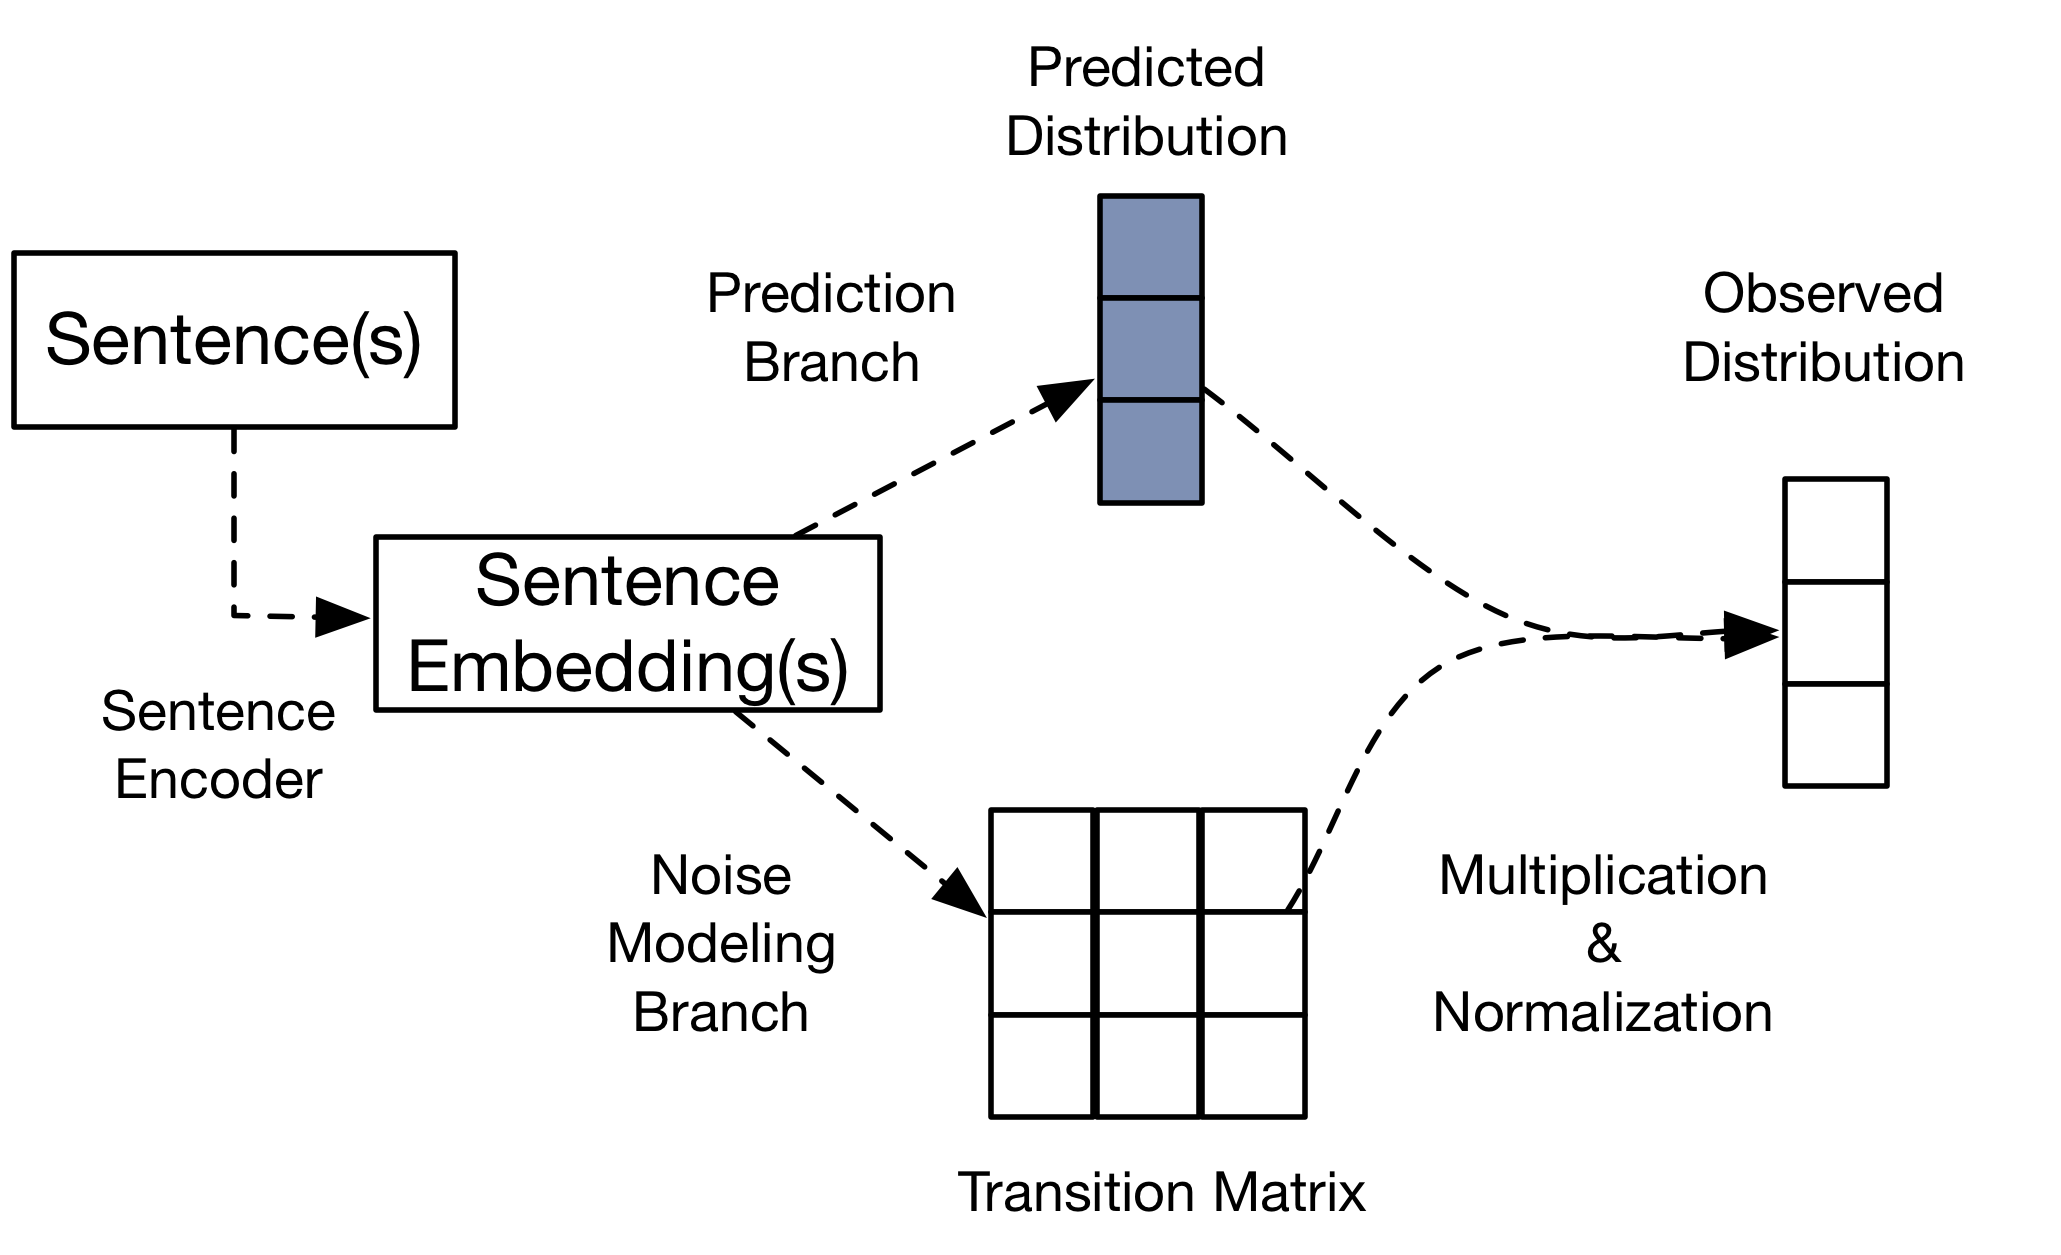
\includegraphics[width=8cm]{denoise_framework.png}	
\caption{The architecture of our denoising model}
\label{fig: denoise_framework}
\end{center}
\end{figure}

The overview of our model is shown in Figure \ref{fig: denoise_framework}. First, the input sentence (or sentence bag) is passed to a sentence encoder to get sentence embedding(s). After that, the model is split into two branches. The prediction branch generates the predicted relation distribution $\mathbf{p}$ of the input sentence (or sentence bag). The noise modeling branch generates the transition matrix $\mathbf{T}$. Finally, the predicted distribution is multiplied by the transition distribution to generate the observed relation distribution $\mathbf{o}$. The predicted relation distribution $\mathbf{p}$ is the output of the model while the observed relation distribution $\mathbf{o}$ is used to simulate the relation assigned by distant supervision. In this way, the noise is modeled by the transition matrix and the real prediction is protected from the influence of the noise.

\subsection{Sentence Encoder}
\todo{add distance embedding}
Similar to previous researches in relation extraction, we also use the piecewise convolutional neural network (PCNN) model \cite{zeng2015distant} as our sentence encoder. The PCNN model first divides the input sentence into three pieces by the subject and the object. After that, it will apply convolutional neural network (CNN) to each piece to calculate the piece embedding. The final sentence embedding is the concatenation of the embeddings of the three pieces.

\subsection{Prediction Branch}
The prediction branch can be implemented by the prediction part of almost all the relation extraction neural network models. As for sentence level models, we use the settings of \cite{luo2016temporal}. Specifically, we first feed the sentence embedding to a full connection layer, and use softmax classifier for relation classification. As for bag level models, the key problem is how to aggregate the embeddings of each sentence in a bag. Similar to \cite{lin2016neural}, we experiment with two settings: average aggregation and attention aggregation. The average aggregation calculates the bag embedding $\mathbf{s}$ by averaging the embeddings of each sentence, and the resultant bag embedding is fed to a softmax classifier for relation classification. The attention aggregation method \cite{lin2016neural} calculates bag embeddings with respect to each relation. For example, the bag embedding with respect relation $j$ is:
\begin{equation}
\mathbf{s}_j = \sum_i^{n}{\alpha_{ij} \mathbf{x}_{i}}
\end{equation}
\begin{equation}
\alpha_{ij} = \frac{exp(\mathbf{x}_{i}^T \mathbf{Ar}_j))}{\sum_{i}{exp(\mathbf{x}_{i}^T \mathbf{Ar}_j)}}
\end{equation}
where and $\alpha_{ij}$ is the attention over sentence $i$ with respect to relation $j$, $\mathbf{A}$ is a diagonal matrix and $\mathbf{r_j}$ is the randomly initialized embedding of relation $j$. The resultant bag embedding is fed to a softmax classifier to predict the probability of relation $j$.

\subsection{Noise Modeling Branch}
Parallel to the prediction branch, the noise modeling branch calculates a transition matrix dynamically for each sentence (or sentence bag) to model its noise pattern.

\paragraph{Sentence Level Transition Matrix}
As for sentence level models, the sentence embedding $\mathbf{x}$ is passed to another full connection layer to obtain the sentence embedding $\mathbf{x}_n$ used specifically for the noise branch. After that, the transition matrix $\mathbf{T}$ is calculated using a softmax classifier:
\begin{equation}
T_{ij} = \frac{exp({(\mathbf{w}_t^{ij})^T \mathbf{x}_n + b_t})}{\sum_{j=1}^{|\mathbb{C}|}{exp({(\mathbf{w}_t^{ij})^T \mathbf{x}_n + b_t}})}
\end{equation}
where $T_{ij}$ is the conditional probability that this sentence is labeled as relation $j$ by distant supervision given the true relation is $i$, $\mathbf{w}_t^{ij}$ is the weight vector for this situation, $b_t$ is a scalar bias and $|\mathbb{C}|$ is the number of relations.

\paragraph{Bag Level Transition Matrix}
As for bag level models, we first use the attention mechanism to calculate the bag embedding with respect to each relation:
\begin{equation}
\mathbf{s}_{j} = \sum_i^{n}{\alpha_{ij} \mathbf{x}_{i}}
\end{equation}
\begin{equation}
\alpha_{ij} = \frac{exp(\mathbf{x}_i^T \mathbf{r}_t^j)}{\sum_i^n{exp(\mathbf{x}_i^T \mathbf{r}_t^j)}}
\end{equation}
where $\mathbf{s}_j$ is the bag embedding with respect to relation $j$, $\mathbf{x}_i$ is the embedding of sentence $i$, $\alpha_{ij}$ is the attention value and $\mathbf{r}_t^j$ is another randomly initialized embedding of relation $j$ used specifically for noise modeling branch. 

Then the transition matrix $\mathbf{T}$ is calculated by:
\begin{equation}
T_{ij} = \frac{exp({(\mathbf{r}_t^j)^T \mathbf{s}_i + b_t})}{\sum_{j=1}^{|\mathbb{C}|}{exp((\mathbf{r}_t^j)^T \mathbf{s}_i + b_t})}
\end{equation}
where $\mathbf{s}_i$ is the bag embedding with respect to relation $i$, $\mathbf{r}_t^j$ is the embedding of relation $j$ mentioned above, and $b_t$ is a scalar bias. 

Note that the softmax function guarantees that each row of the transition matrix $\mathbf{T}$ sums to 1 in both sentence level and bag level models. Here $T_{ij}$ represents the conditional probability that the relation labeled by distant supervision is $j$ given the true relation is $i$.


\subsection{Observed Relation Distribution}
Given the predicted relation distribution $\mathbf{p}$ calculated by the prediction branch, and the transition matrix $\mathbf{T}$ calculated by the noise modeling branch, the observed relation distribution $\mathbf{o}$ is calculated by:
 \begin{equation}
\mathbf{o} = \mathbf{T}^T \bm\cdot \mathbf{p}
 \end{equation}
 \begin{equation}
 \label{norm_o}
 o_i = \frac{o_i}{\sum_i{o_i}}
 \end{equation}
 where $\bm\cdot$ represents dot product and Equation \ref{norm_o} normalizes the elements of $\mathbf{o}$ so that $\sum_i{o_i}=1$
 
Different from previous works that use the predicted relation distribution $\mathbf{p}$ to directly match the relation labeled by distant supervision. We instead use $\mathbf{o}$ to match the relation assigned by distant supervision. In this way, we can model the procedure of how the noisy label is produced and thus protect our prediction $\mathbf{p}$ from the influence of the noise.

Note that the noise modeling branch and $\mathbf{o}$ is only used in the training phase. In the test phase, we only use the prediction brach and take the predicted relation distribution $\mathbf{p}$ as our output.

\section{Training Procedure} 
Note that if we apply the transition matrix model directly to the training data, there is no incentive for the predicted relation distribution $\mathbf{p}$ to model the true relation distribution, instead it will probably be treated as a normal hidden layer. In this section, we show how to combine the curriculum learning framework and a novel normalization strategy to solve this problem. We describe the training procedure in the situation with and without the prior knowledge of the data quality.

\subsection{Curriculum Learning over Dataset}
\todo{describe the curriculum learning for bag level methods in experiment part}
The basic idea of curriculum learning is simple: start with the easiest aspect of a task, and level up the difficulty gradually. 

The most straight forward way to build a curriculum is by controlling the training data. If we have both reliable and unreliable data, we can first train the prediction branch on the reliable data for $t_1$ epochs so that the prediction branch will have the basic classification ability. Then we add the unreliable data as well as the noise modeling branch. In this way, the prediction branch will already possess the tendency to predict true relation distribution before exposed to noisy data. 

Specifically, in the dataset of \cite{luo2016temporal}, we have three subsets with decreasing reliability. We first train the prediction branch on the reliable subset for $t_1$ epochs. After that, we add the less reliable subset and the most unreliable subset consecutively and train for $t_2$ and $t_3$ epochs respectively (for simplicity, here we set $t_1=t_2=t_3$).

\subsection{Trace Normalization}
The curriculum learning method above only works when we know which data are reliable. Here we introduce how to use trace normalization to control the behavior of the transition matrix and how to use this method to build a more general curriculum in the next section.
 
Intuitively, if the noise is small, the transition matrix $\mathbf{T}$ will tend to become an identity matrix. Therefore, we can utilize our prior knowledge of the data quality by controlling the similarity between $\mathbf{T}$ and identity matrix. In the situation where we do not know which data are reliable, we can first force the transition matrix to be similar to identity matrix until the prediction branch is roughly trained. Then by gradually relax the constraint, the model will gradually learn to model the noise in the dataset.

Specifically, since each row of $\mathbf{T}$ sums to 1, the similarity between the transition matrix and the identity matrix can be represented by the trace of the transition matrix $\mathbf{T}$. The larger the $trace(\mathbf{T})$ is, the smaller the elements that do not lie in the diagonal are, and the similar the transition matrix $\mathbf{T}$ is to identity matrix.

Since we have the prior knowledge of the quality of the three subsets of the dataset of Luo et.al, we can further use three hyper-parameters $\{\beta_1, \beta_2, \beta_3\}$ to control the $trace(\mathbf{T})$ of the three subsets. For reliable subset, we want $trace(\mathbf{T})$ to be large (negative $\beta_1$) so that the element values of $\mathbf{T}$ will be centralized to the diagonal. As for unreliable subsets, we want the $trace(\mathbf{T})$ to be small (positive $\beta_2$ and $\beta_3$) so that the element values of their transition matrices will be diffusive. Note that this method only works for sentence level models, since reliable sentences and unreliable ones are all aggregated into a sentence bag in bag level models and therefore we can not determine which bag is reliable. and which is not. We use cross entropy as our basic loss function, and the loss function of the sentence level model is defined as follows:

\begin{equation}
\begin{aligned}
J(\theta)=\sum_{i=1}^3{\sum_{j=1}^{N_i}{-log(o_{ijy_{ij}})}} + \beta_i trace(\mathbf{T}_{ij})
\end{aligned}
\end{equation}
where $\theta$ represents all the parameters in our model, $i$ is the index of the three subsets, $j$ is the index of sentence, $\mathbf{T}_{ij}$ is the transition matrix of sentence $s_{ij}$, $y_{ij}$ is the relation assigned by distant supervision for sentence $s_{ij}$, and $o_{ijy_{ij}}$ is the probability that the observed relation for sentence $s_{ij}$ is $y_{ij}$.

\subsection{Curriculum Learning over Noise Modeling Strength}
As for bag level models, and in the situation where we do not have prior knowledge of the data quality, we can build a curriculum by controlling our expectation for the model to model the noise. Specifically, the loss function is defined as follows:

\begin{equation}
\begin{aligned}
J(\theta)	&=\sum_{i=1}^N{-(\alpha log(o_{iy_{i}}) + (1-\alpha) log(p_{iy_{i}}))} \\
&+ \beta trace(\mathbf{T}_{i})
\end{aligned}
\end{equation}
where $0\le\alpha\le1$, $y_i$ is the relation assigned by distant supervision for sentence $s_i$, $o_{iy_{i}}$ and $p_{iy_{i}}$ is the probability that the observed and predicted relation for setnence $s_i$ is $y_i$. \todo{polish the statement before} Instead of only using the observed relation distribution $\mathbf{o}$ to simulate the relation labeled by distant supervision, we use the linear combination of the cross entropy of both the observed relation distribution $\mathbf{o}$ and the predicted relation distribution $\mathbf{p}$. 

At the start of the training, we set $\alpha=1$ and $\beta<0$, which means we do not expect the model to model the noise (easy part of the problem). As the training proceeds, the prediction branch gradually learns the basic prediction ability. Therefore, we decrease $\alpha$ and the absolute value of $\beta$ by $d$ every $\tau$ epochs to gradually lead the model to learn to model the noise.  

\subsection{Constraint Transition Matrix}
Recall that the bag level noise mainly consists of false negative and false positive, but our transition matrix also has the ability to model the confusion among positive relations. To prevent overfitting and make the model concentrate on the false negative and false positive noise, we restrict the transition matrix for bag level models so that only the diagonal, the first column and the first row of the transition matrix do not equal to zero (assume the index of \emph{no-relation} is 0).  


\section{Experiments}
\subsection{Data Set}
We experiment our model on two datasets. The first one is proposed by \cite{luo2016temporal} and aims at extraction relations between entity and time (\emph{time RE data}). The dataset is constructed by aligning Wikidata triples with Wikipedia corpus. Based on the granularity of the time expression in the sentence, this dataset can be split into 3 subsets with different levels of reliability. The reliable subset is used as basic training data, validation data and test data which contains 22,214, 2,776 and 2,771 positive sentences respectively. The two less reliable subset contains 2,094 and 53,469 positive sentences and are used as additional training data. Negative data are constructed with two heuristic strategies. We use this dataset because this is a public dataset on relation extraction that has both reliable and unreliable data, which is suitable for all of our experiment settings.

We also conduct our experiment on the dataset proposed by \cite{riedel2010modeling}, which is a commonly used dataset in relation extraction (\emph{entity RE}). This dataset is generated by aligning triples in Freebase with the New York Times corpus (NYT corpus). The training data contains 522,611 sentences and 281,270 entity pairs. The test set contains 172,448 sentences and 96,678 entity pairs. We experiment our bag level models in this dataset to see the generalization ability of our transition matrix model.


\subsection{Hyper-parameters}
\paragraph{Sentence Level Model}
We experiment our sentence level model on time RE data. We use 100-dimensional word embedding pre-trained using GloVe \cite{pennington2014glove} on Wikipedia and Gigaword, and 20-dimensional vector for distance embedding. The convolution window is 3 and the number of convolution kernels is 200. The size of the full connection layer is also 200. As for training, we use stochastic gradient descend (SGD) for optimization with batch size 20, learning rate 0.1. We also use dropout with probability 0.5 upon the sentence embedding. Each phase of the curriculum learning over dataset contains 15 epochs. The trace normalization parameters for three subsets are $\beta_1=-0.01$, $\beta_2=0.01$ and $\beta_3=0.1$ (the ratio of $\beta_3$ and $\beta_2$ is fixed to 10 and 5 when tuning hyper-parameters).

\paragraph{Bag Level Model}
The parameters of the bag level model is almost the same as the sentence level model on time RE data, except that the learning rate is 0.01. As for entity RE data, our settings for prediction branch is similar to \cite{lin2016neural}. The word embedding is of dimension 50 and is pre-trained on the NYT corpus using word2vec\footnote{\url{ https://code.google.com/p/word2vec/}}. The convolution window is 3 and the number of convolution kernels is 256, distance embedding size is 5, batch size is 16 and learning rate is 0.01. For all the bag level models, the linear combination parameter $\alpha$ is 1 and trace normalization parameter $\beta$ is -0.1 at the start of training. We experiment with decay rate \{0.95, 0.9, 0.8\} and decay step \{3, 5, 8\}. We find that using decay rate 0.9 and decay step 5 performs well in most situations.

\begin{figure}[htbp]
\begin{center}
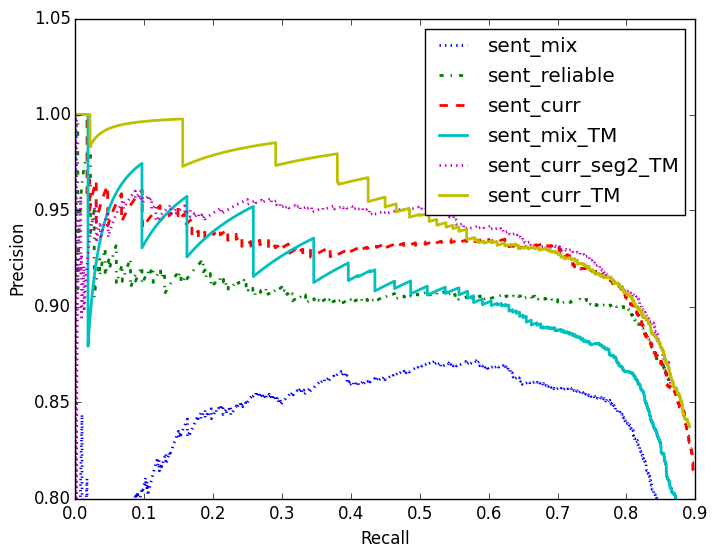
\includegraphics[width=0.9\linewidth]{sent_time_exp_overall.png}
\caption{Sentence Level Results on Time RE}
\label{fig: sent_luo}
\end{center}
\end{figure}

\subsection{Results on Time RE Data}
We exhibit the results in the form of precision recall curves (PR curves). 

\paragraph{Sentence Level Models}
The results of sentence level models is shown in Figure \ref{fig: sent_luo}. We can see that the performance of the model trained on all subsets mixed together (\emph{sent\_mix}) is very bad, which is significantly worse than the model trained only on the reliable subset (\emph{sent\_reliable}). This shows that the noise problem is innegligible and have bad influence on the training of the model. However, with the help of transition matrix, the model obtains the ability of modeling noise (\emph{sent\_mix\_TM}), which significantly improves the performance of the model. By using the reliable subset first and gradually adding less reliable data (\emph{sent\_curr}), we can see that the model can actually make use of the noisy data and performs better than the model trained only on the reliable subset. If we further use the transition matrix under the curriculum learning framework (\emph{sent\_curr\_TM}), the transition matrix will model the noise better and further improve the model performance. Apart from the experiments above, we also experiment our model in the situation where all the unreliable data are merged into one subset (\emph{sent\_seg2\_curr\_TM}), which means there are only two subsets: reliable subset and unreliable subset. We conduct this experiment because this setting will reduce the hyper-parameters and make the training easier to perform. We can see the, although this setting is not as good as using the full information of the data quality (using 3 subsets), it still has reasonable performance and also significantly outperforms the model which only use curriculum learning over dataset.


\begin{figure*}[htbp]
\centering
\subfigure[Attention Aggregation]{
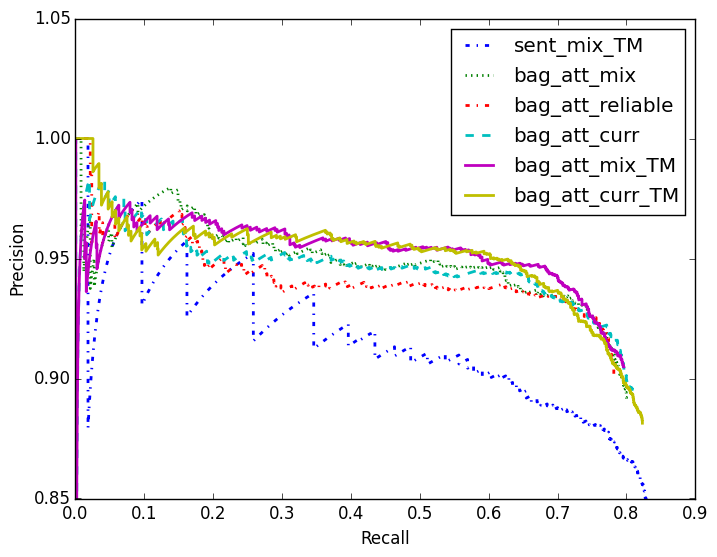
\includegraphics[width=0.45\linewidth]{bag_att_exp_overall.png}
\label{fig: bag_att_luo}
}
\subfigure[Average Aggregation]{
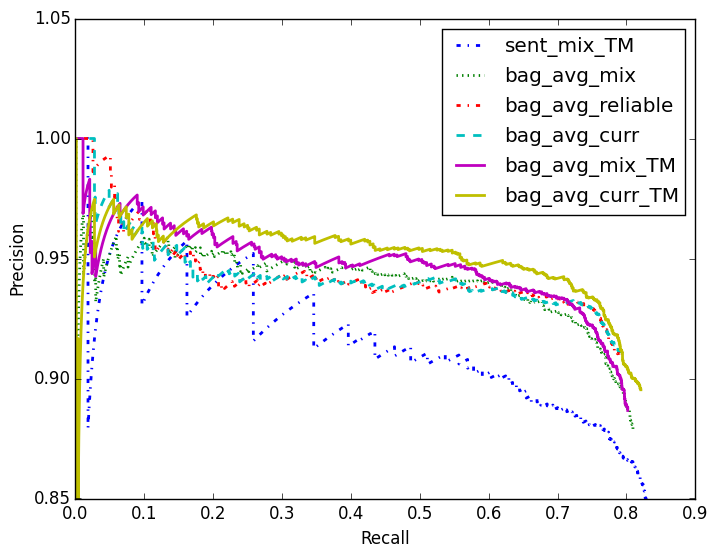
\includegraphics[width=0.45\linewidth]{bag_avg_exp_overall.png}
\label{fig: bag_avg_luo}
}
\caption{Bag Level Results on Time RE}
\label{fig: results_on_luo}
\end{figure*}

\paragraph{Bag Level Attention Aggregation Models}
The results of the bag level models with attention aggregation is shown in Figure \ref{fig: bag_att_luo}. We can see that the basic bag level attention aggregation model (\emph{bag\_att\_mix}) performs very good and significantly outperforms the \emph{sent\_mix\_TM} model. Recall that the bag level model is based on the at-least-one assumption that at least one of the sentences in the sentence bag support the ($subj$, $rel$, $obj$) triple, and the \emph{sent\_mix\_TM} model do not use any assumption about the dataset. This shows that prior knowledge of the data quality plays an important role in the situation where the dataset is noisy. In the bag level models, the curriculum learning over dataset can be conducted by using only the reliable sentences in the sentence bag, and add unreliable sentences gradually. However, we find that using only reliable subset (\emph{bag\_att\_reliable}) or using curriculum learning over dataset alone (\emph{bag\_att\_curr}) does not improve the bag level attention aggregation model. This shows that the less reliable data in the sentence bag may provide additional side information or possibly plays the role of avoiding overfitting. \todo{polish the explanation.} Also note that the at-least-one assumption does not always hold and there are also false negative and false positive problems in bag level. Therefore, we can see that using transition matrix with or without curriculum learning over the dataset (\emph{bag\_att\_curr\_TM} and \emph{bag\_att\_mix\_TM}) all improve the model performance, and the \emph{bag\_att\_curr\_TM} model performs better in the low recall region.

\paragraph{Bag Level Average Aggregation Models}
The results of the bag level models with average aggregation is shown in Figure \ref{fig: bag_avg_luo}. The ranking of each setting is similar to the attention aggregation models. One interesting thing is that our transition matrix method improves the average aggregation models more significantly than the attention aggregation models. Note that the average aggregation model actually do not have good ability of handling sentence level noise. Therefore, the unhandled sentence level noise may further propagate to the bag level, which gives the transition matrix more chance to help model the noise. Also note that the \emph{bag\_avg\_curr\_TM} model significantly outperforms the \emph{bag\_avg\_mix\_TM}, this shows that curriculum learning over dataset helps the transition matrix more when the noise is more severe.
 
\begin{figure}[htbp]
\begin{center}
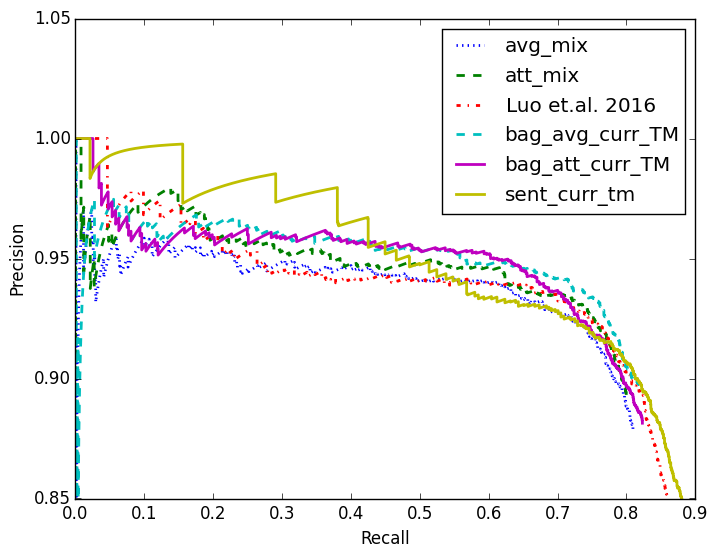
\includegraphics[width=0.9\linewidth]{best_cmp_exp_overall.png}
\caption{Comparison on Time RE}
\label{fig: cmp_luo}
\end{center}
\end{figure}
 
\paragraph{Comparison}
\todo{polish this part} 
The comparison of the best settings of each model family is shown in Figure \ref{fig: cmp_luo}. We can see that all of our models outperforms the model of \cite{luo2016temporal}. With the help of transition matrix, although the basic version of average aggregation is not as good as attention aggregation, its transition matrix version is similar to the attention aggregation. Also note that although the sentence level models trained on mixed data do not perform very good, the sentence level model can use transition matrix to model the sentence level noise and thus performs best in all these models. Recall that the transition matrix can model the noise rather than just reduce the influence of noisy sentences as in bag level models, the sentence level model actually has the ability to make use of the noisy data. This shows that sentence level noise is more important than the bag level noise in relation extraction, and modeling noise works better than just trying to reducing the influence of noise.


\begin{figure}[htbp]
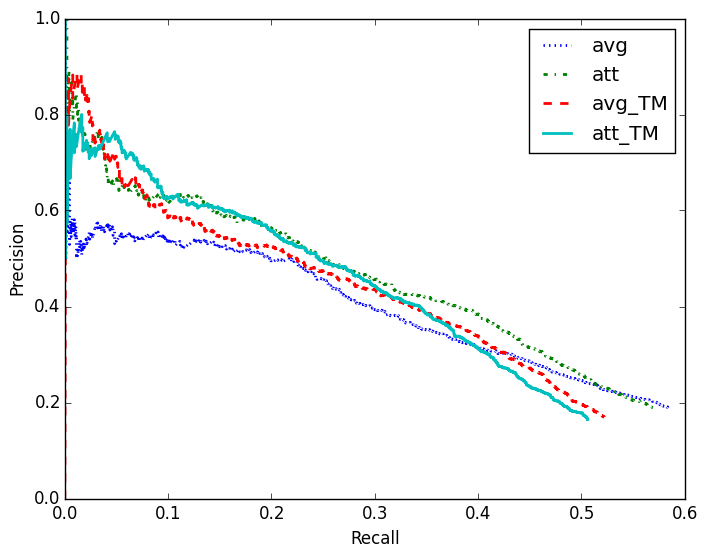
\includegraphics[width=0.9\linewidth]{re_att_avg_cmp_exp.png}
\caption{Results on Dataset of Riedel et.al.} 
\label{fig: Riedel_res}
\end{figure}

\subsection{Performance on Entity RE Data}
To show the generalization ability of our proposed transition matrix method, we also conduct experiments on the entity RE dataset proposed by \cite{riedel2010modeling}, which is a commonly used dataset in relation extraction. We implement the average aggregation method (\emph{avg}) and the attention aggregation method (\emph{att}) proposed by \cite{lin2016neural} as well as the corresponding transition matrix version (\emph{avg\_TM} and \emph{att\_TM}). The results are shown in Figure \ref{fig: Riedel_res}. We can see that, since the average aggregation method do not have good ability in handling sentence level noise, it performs significantly worse than the attention aggregation method. Similar to the results in time RE data, since the unhandled sentence level noise propagates to the bag level, which makes the bag level noise become more severe, the transition matrix has more chance to model the noise. Therefore, the \emph{avg\_TM} model significantly outperforms the \emph{avg} model. As for attention aggregation, this model already have good ability in reducing the impact of sentence level noise. Since the bag level noise is less important than the sentence level noise, the improvement of our transition matrix model is limited, which only improves the model on the low recall part. Note that the low recall part corresponds to high precision, which is more useful than the rest of the extraction results in practice. Therefore, our transition matrix method is also useful in this situation.

\iffalse
\begin{figure*}[htbp]
\centering
\subfigure[Overall PR Curves]{
\includegraphics[width=0.475\linewidth]{reg_exp_overall.png}
\label{fig: reg_overall_pr_curve}
}
\subfigure[Small Relation PR Curves]{
\includegraphics[width=0.475\linewidth]{reg_exp_small.png}
\label{fig: reg_small_rel_pr_curve}
}
\caption{Imapct of Regularization Weights} 
\label{fig: reg_PR_curve}
\end{figure*}
\fi

\section{Conclusion}
\todo{re-write}


\clearpage

% include your own bib file like this:
%\bibliographystyle{acl}
%\bibliography{acl2017}
\bibliography{acl2017}
\bibliographystyle{acl_natbib}



\end{document}
